\documentclass[a4paper, 11pt]{article}

\usepackage[utf8]{inputenc}
\usepackage[english]{babel}

\usepackage{hyperref}

\usepackage{standalone}

\usepackage{lscape}

\usepackage{graphicx}
\usepackage{subfig}
\usepackage{tikz}
\usetikzlibrary{decorations.pathreplacing}

\usepackage{floatrow}
\captionsetup{labelsep=period}

\usepackage{listings}

\usepackage{fullpage}

\begin{document}
	\begin{centering}
		\Large{\textbf{Progress Report}}\\
		\large{\today}
~\\
		Oussama ENNAFII\\
		Directors: Cl\'ement Mallet \& Florent Lafarge \\
		Advisor: Arnaud Le Bris \\

	\end{centering}


	\section{The Dataset:}
	\subsection{Considerations:}
~\\

	We have decided earlier in June to work on Nantes and Dijon in addition to
	Elancourt. As I explained later, the $3DS$ data for these regions are not
	well formated so that I can retrieve the building entities. In order to
	establish first a whole pipeline. I will deal with those regions later using
	the $CityGML$ data. In consequence, I will continue to work on Elancourt
	only, for now.\\

	I have also relabelled the zone I had labelled before. That is due to the fact
	that the taxonomy has evolved during the annotation. I have used $QGIS$ to
	annotate buildings' projected facets based on errors they showed.\\

	\subsection{Annotated errors:}
~\\


	The errors have been subdivided, based on the labelling, into three classes:

	\begin{itemize}
		\item[-] Unqualified Building Errors: Concerns the buildings that will not
		be taken into consideration,
		\item[-] Building Errors: encompasses the errors that affect the whole
		building (corrensponds roughly to $LoD0$ and $LoD1$ errors),
		\item[-] Facet Errors: concerns errors affecting only a facet.
	\end{itemize}

	\thisfloatsetup{heightadjust=object}
	\begin{figure}
		\begin{center}
			\ffigbox
			{
				\ffigbox[\FBwidth]
				{
					\begin{subfloatrow}[4]
						\captionsetup{labelformat=brace, justification=raggedright}
						\ffigbox[\FBwidth]{\caption{Half Building: only a portion of the building is reconstructed.}\label{fig::half_building}}{\fbox{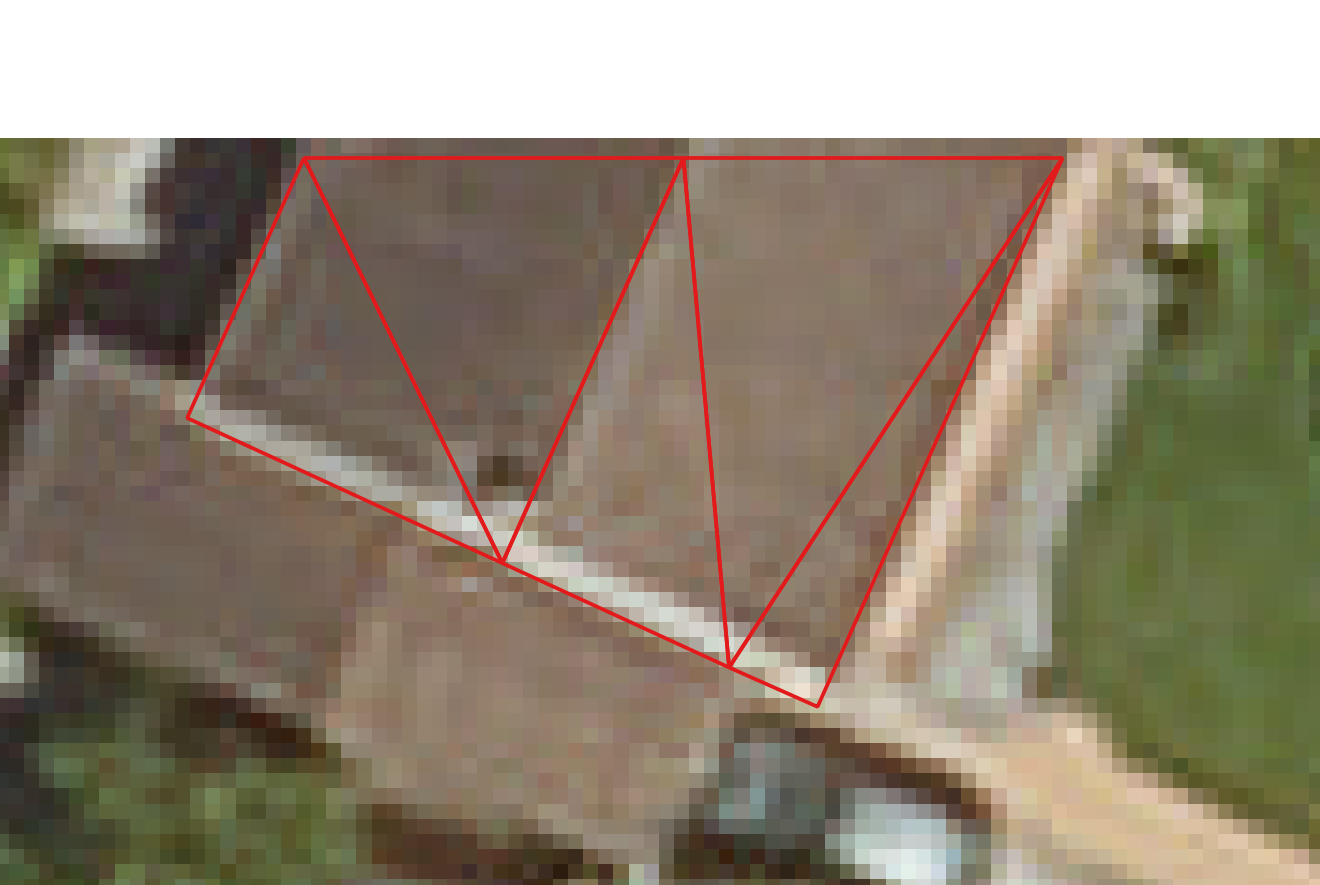
\includegraphics[width=.24\textwidth]{../images/raster/Unqualified_Errors/half_building}}}
						\ffigbox[\FBwidth]{\caption{Changed Building: the building has changed so we cannot qualify it.}\label{fig::changed}}{\fbox{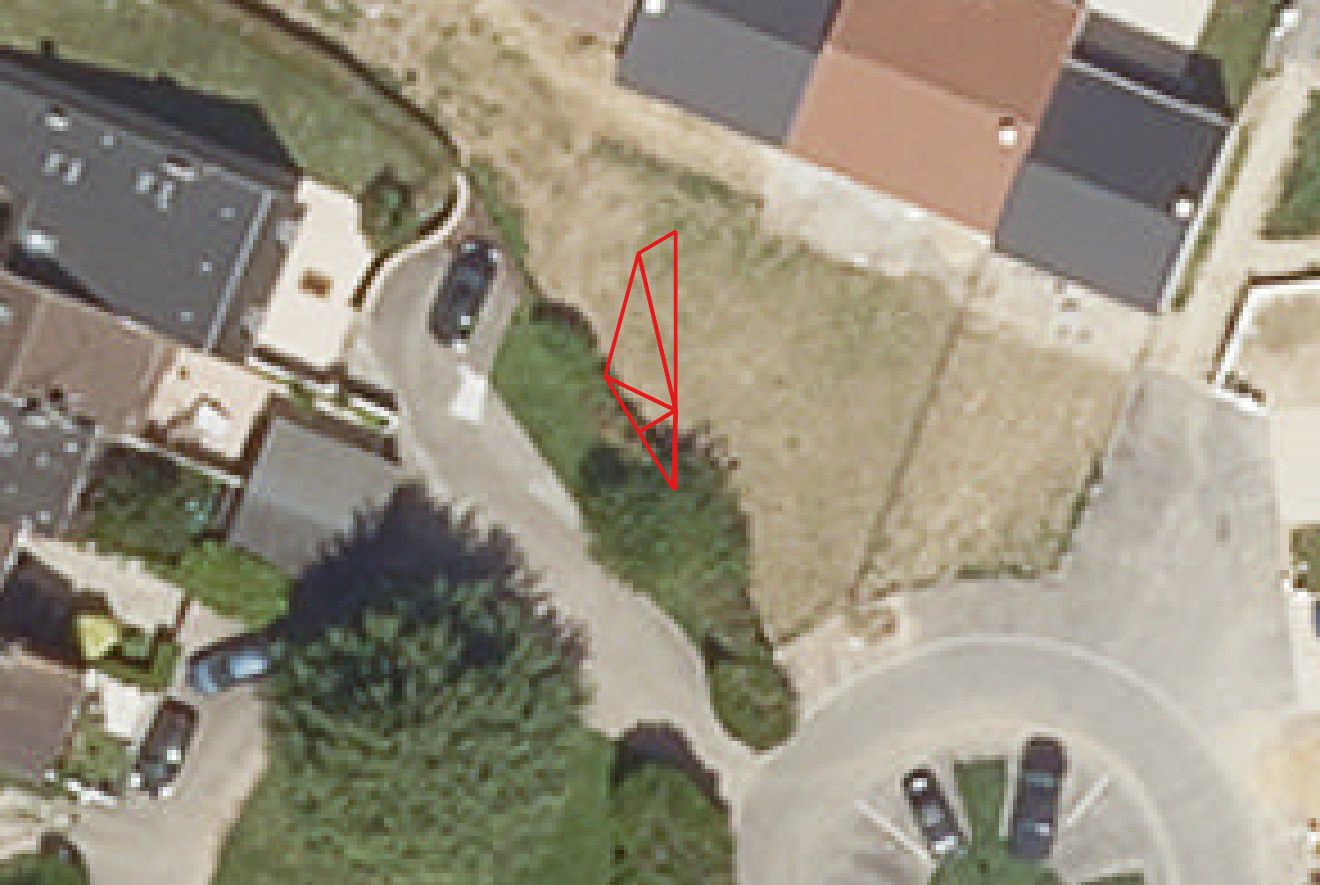
\includegraphics[width=.24\textwidth]{../images/raster/Unqualified_Errors/changed}}}
						\ffigbox[\FBwidth]{\caption{Occlusion: the building is occluded by vegetation here.}\label{fig::occlusion}}{\fbox{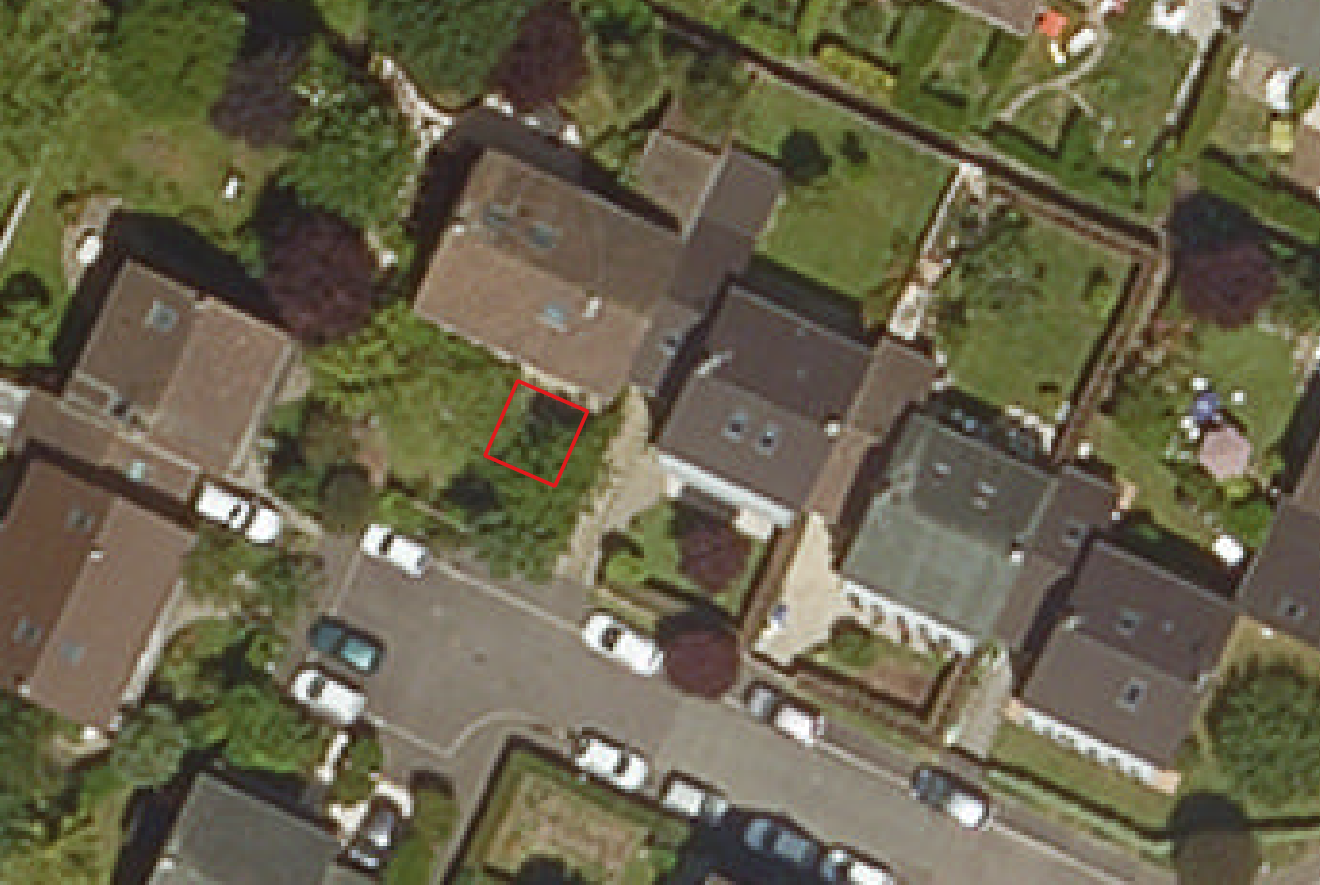
\includegraphics[width=.24\textwidth]{../images/raster/Unqualified_Errors/occlusion}}}
						\ffigbox[\FBwidth]{\caption{Unknown: Unknown shape that cannot be verified on the ground.}\label{fig::unknown}}{\fbox{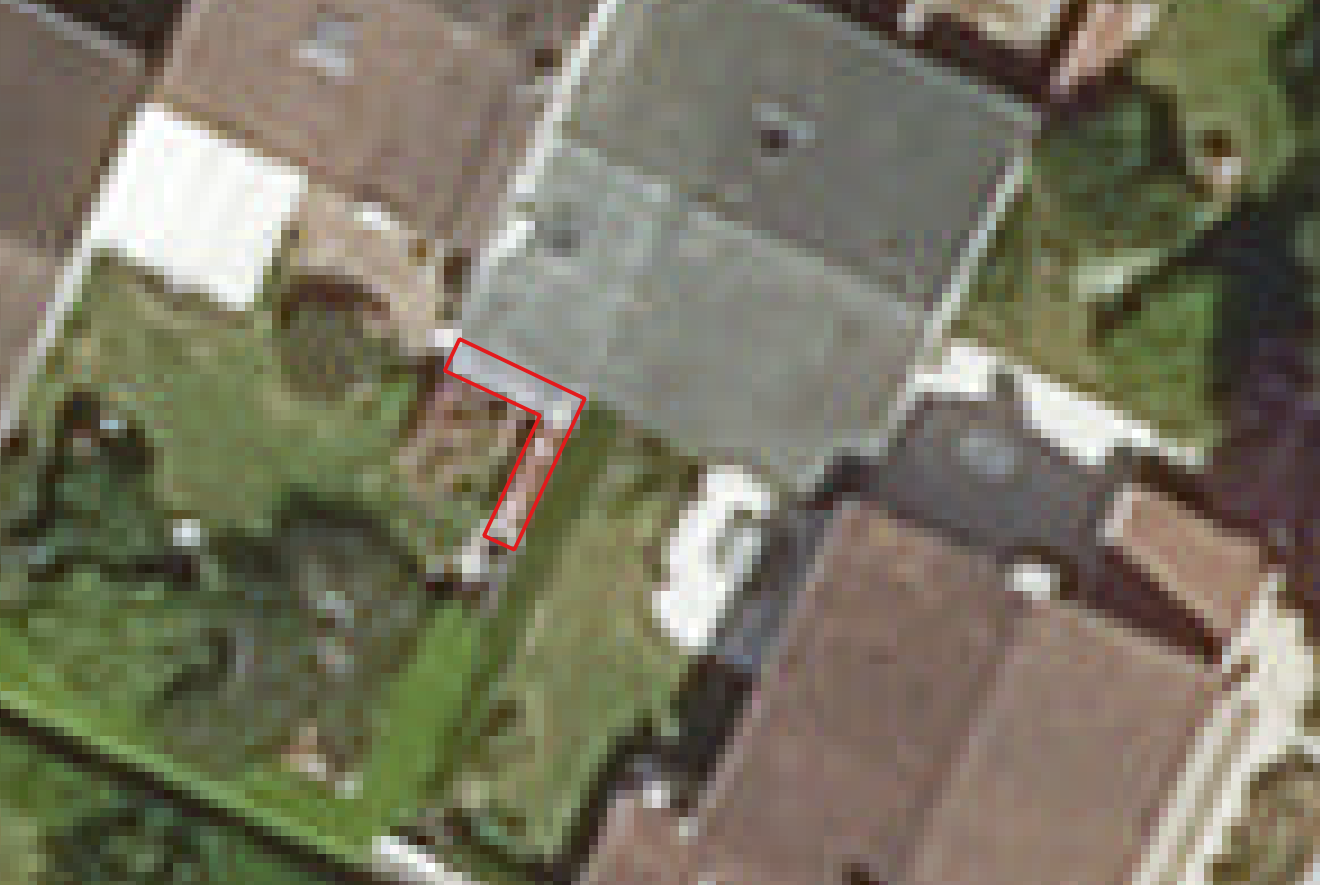
\includegraphics[width=.24\textwidth]{../images/raster/Unqualified_Errors/unknown}}}
					\end{subfloatrow}
				}
				{
					\caption*{\label{fig::unq_samples} (i). Samples of Unqualified building errors.}
				}
				\ffigbox[\FBwidth]
				{
					\begin{subfloatrow}[4]
						\captionsetup{labelformat=brace, justification=raggedright}
						\ffigbox[\FBwidth]{\caption{Under Segmentation: Two or more buildings grouped into one.}\label{fig::under_bul}}{\fbox{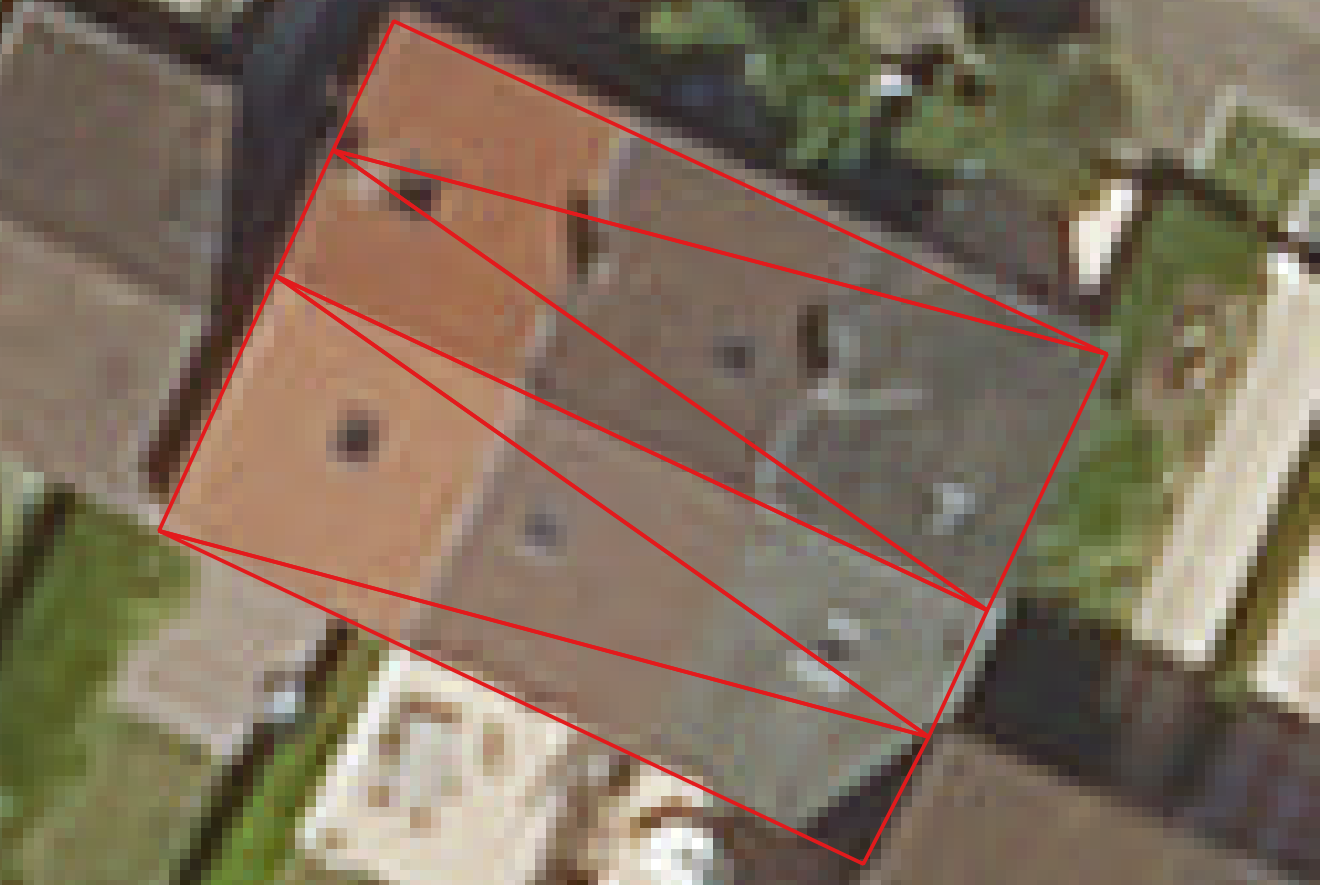
\includegraphics[width=.24\textwidth]{../images/raster/Building_Errors/under_segmentation}}}
						\ffigbox[\FBwidth]{\caption{Over segmentation: One building segmented into two or more buildings.}\label{fig::over_bul}}{\fbox{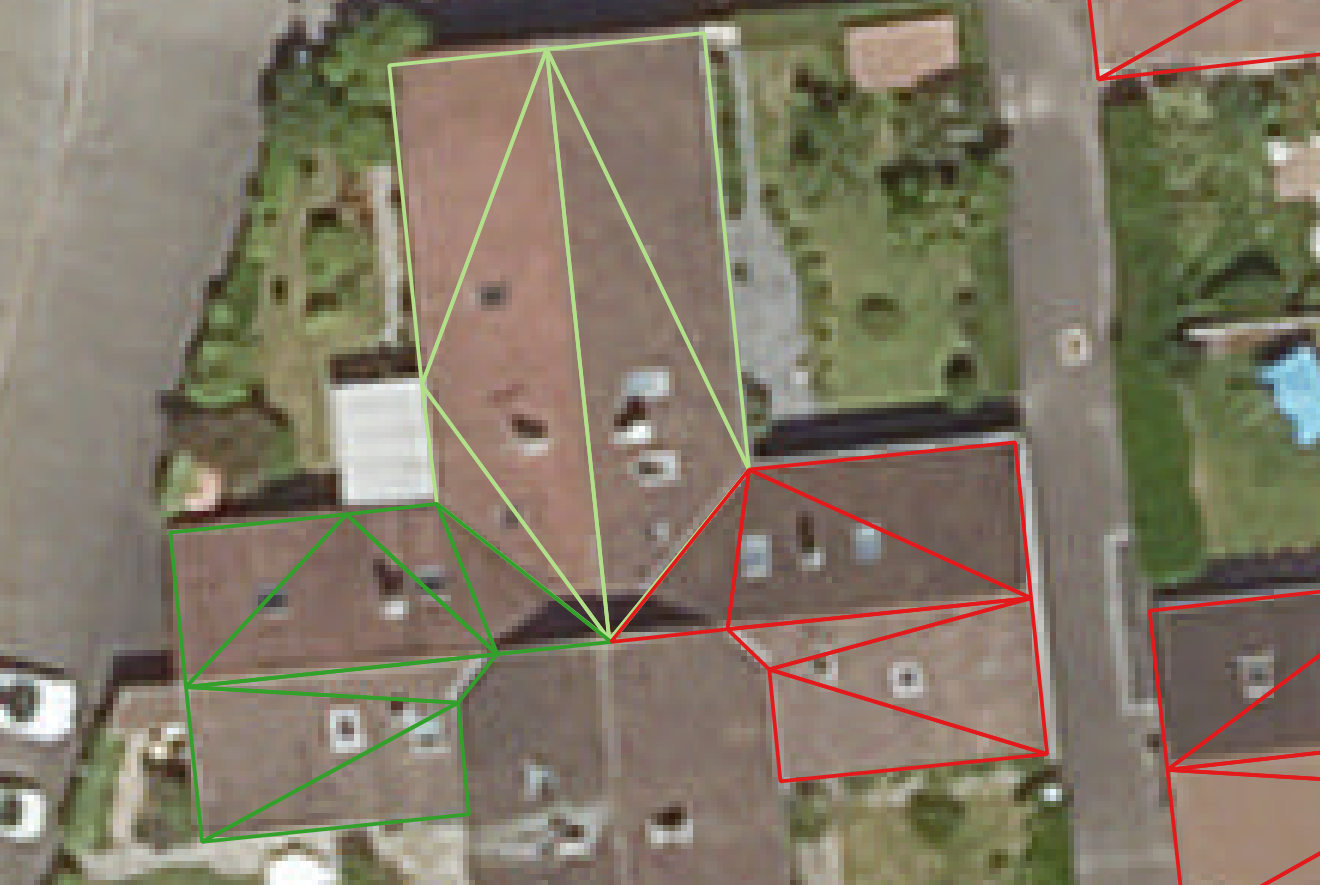
\includegraphics[width=.24\textwidth]{../images/raster/Building_Errors/over_segmentation}}}
						\ffigbox[\FBwidth]{\caption{Footprint: Wrong building footprint.}\label{fig::footprint}}{\fbox{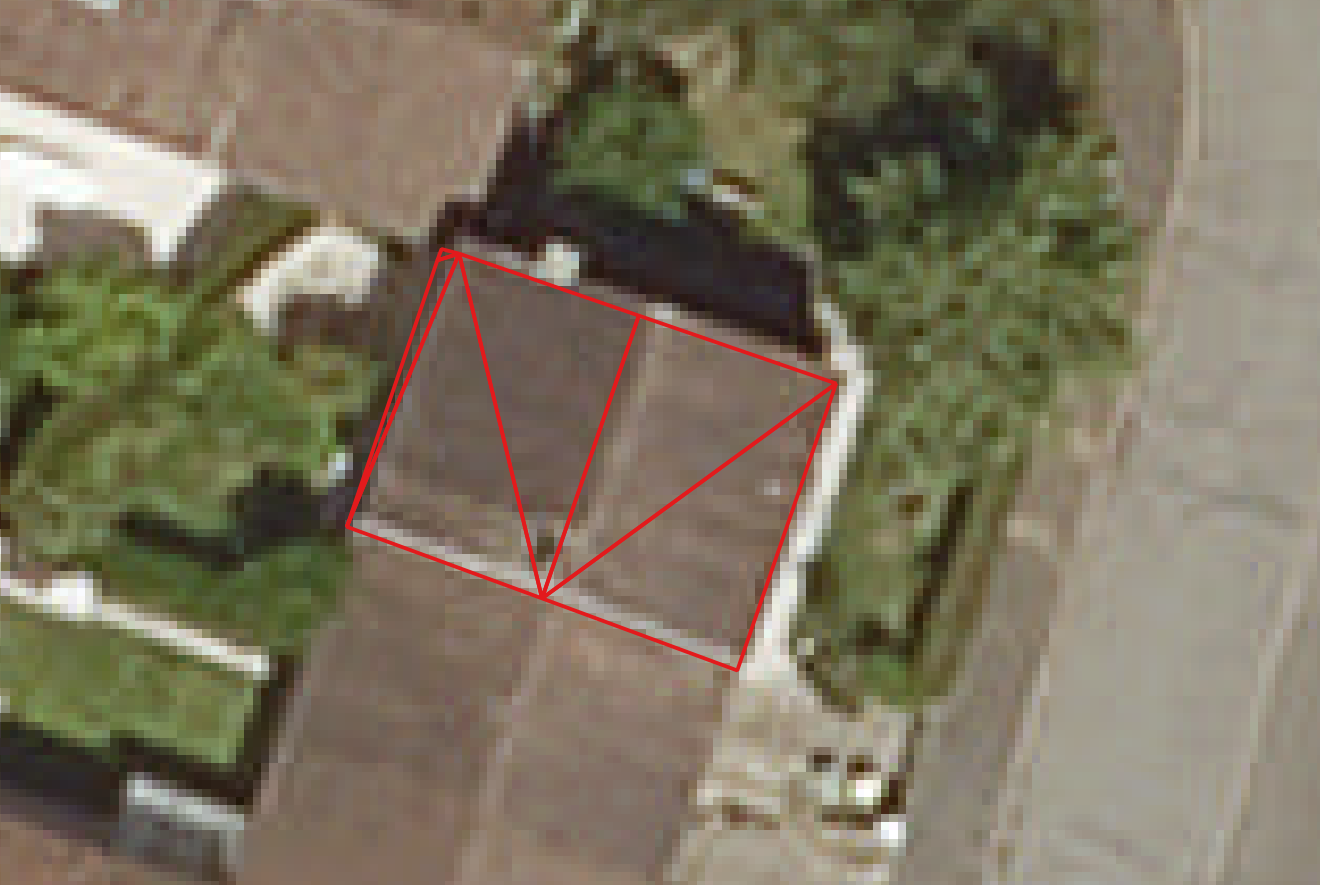
\includegraphics[width=.24\textwidth]{../images/raster/Building_Errors/footprint}}}
						\ffigbox[\FBwidth]{\caption{Altitude: Wrong building height.}\label{fig::too_low}}{\fbox{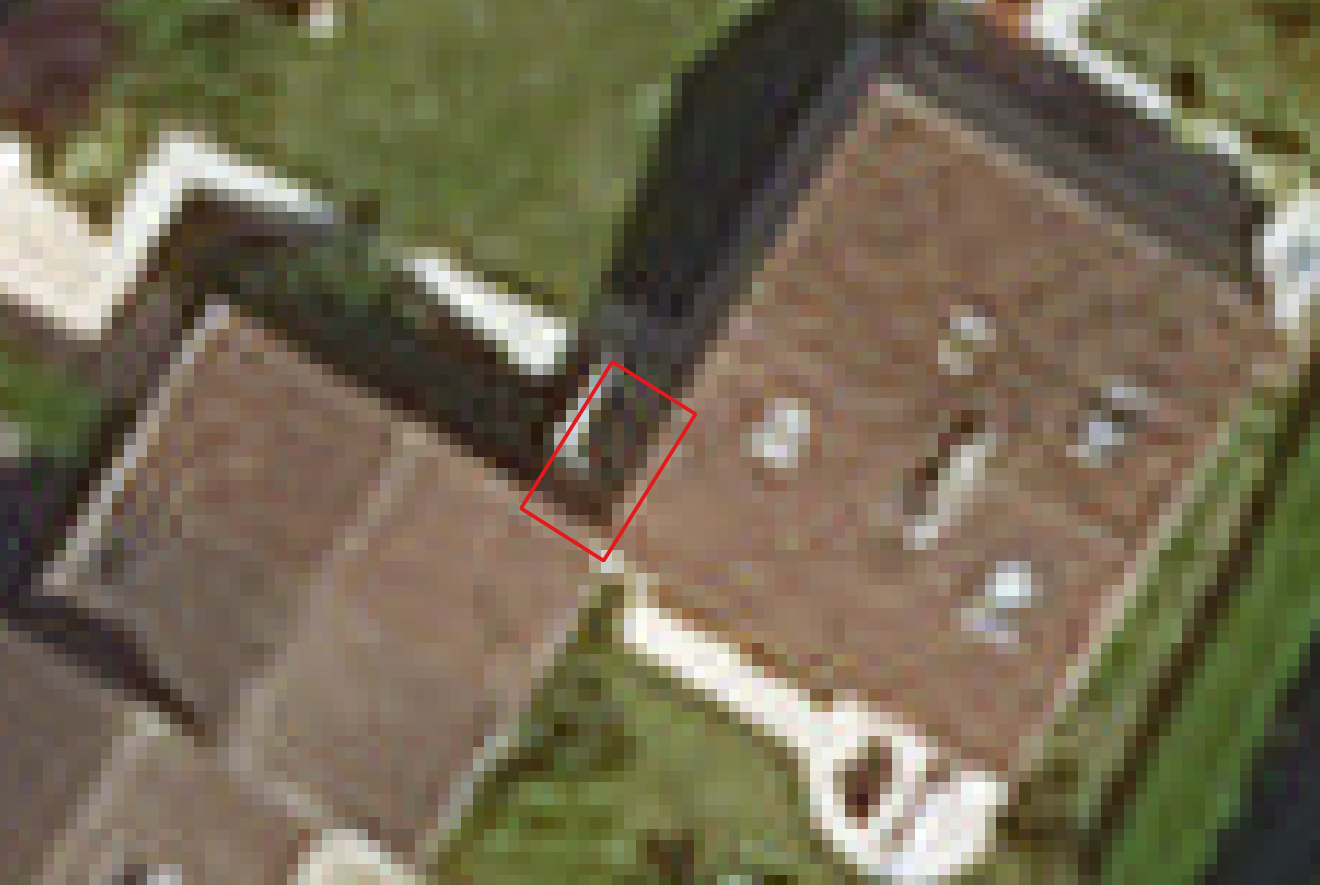
\includegraphics[width=.24\textwidth]{../images/raster/Building_Errors/altimetric}}}
					\end{subfloatrow}
				}
				{
					\caption*{\label{fig::bul_samples} (ii). Samples of Building errors.}
				}
				\ffigbox[\FBwidth]
				{
					\begin{subfloatrow}[4]
						\captionsetup{labelformat=brace, justification=raggedright}
						\ffigbox[\FBwidth]{\caption{Under Segmentation: Two facets or more grouped into one.}\label{fig::under_fac}}{\fbox{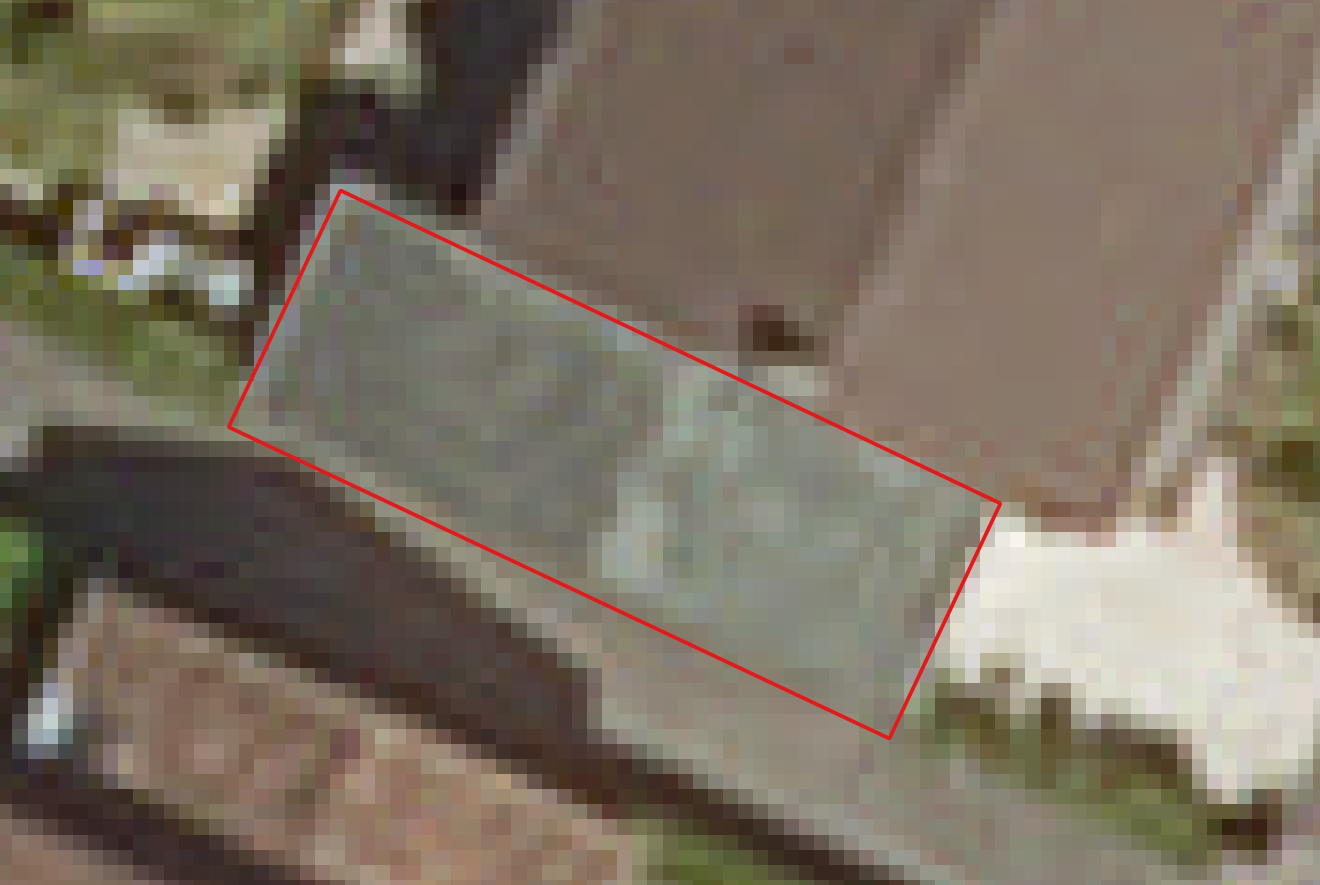
\includegraphics[width=.24\textwidth]{../images/raster/Facet_Errors/under_segmentation}}}
						\ffigbox[\FBwidth]{\caption{Over segmentation: One facet segemented into two or more facets.}\label{fig::over_fac}}{\fbox{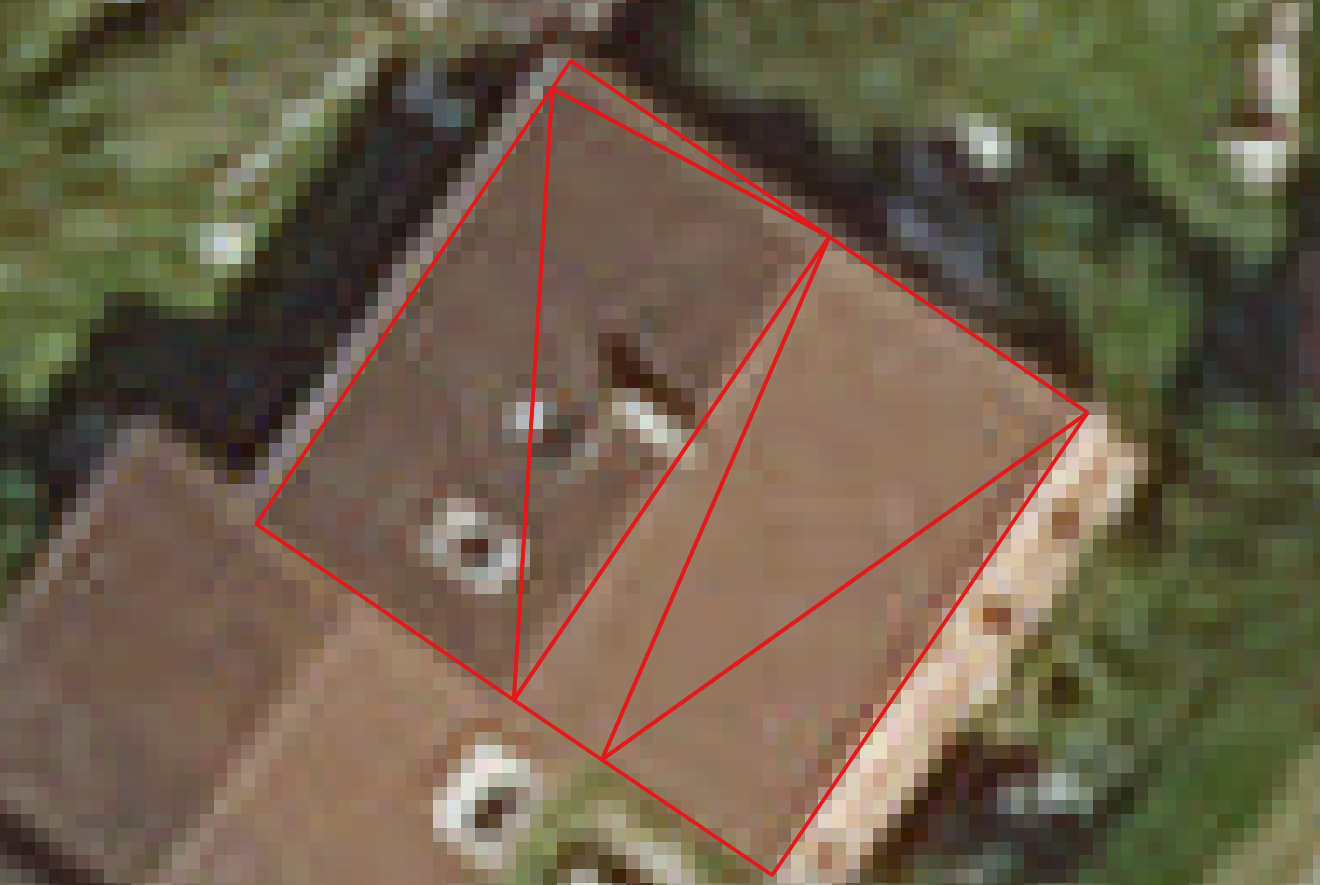
\includegraphics[width=.24\textwidth]{../images/raster/Facet_Errors/over_segmentation}}}
						\ffigbox[\FBwidth]{\caption{Mis Segmentation: Facet edges do not correspond to real ones.}\label{fig::mis}}{\fbox{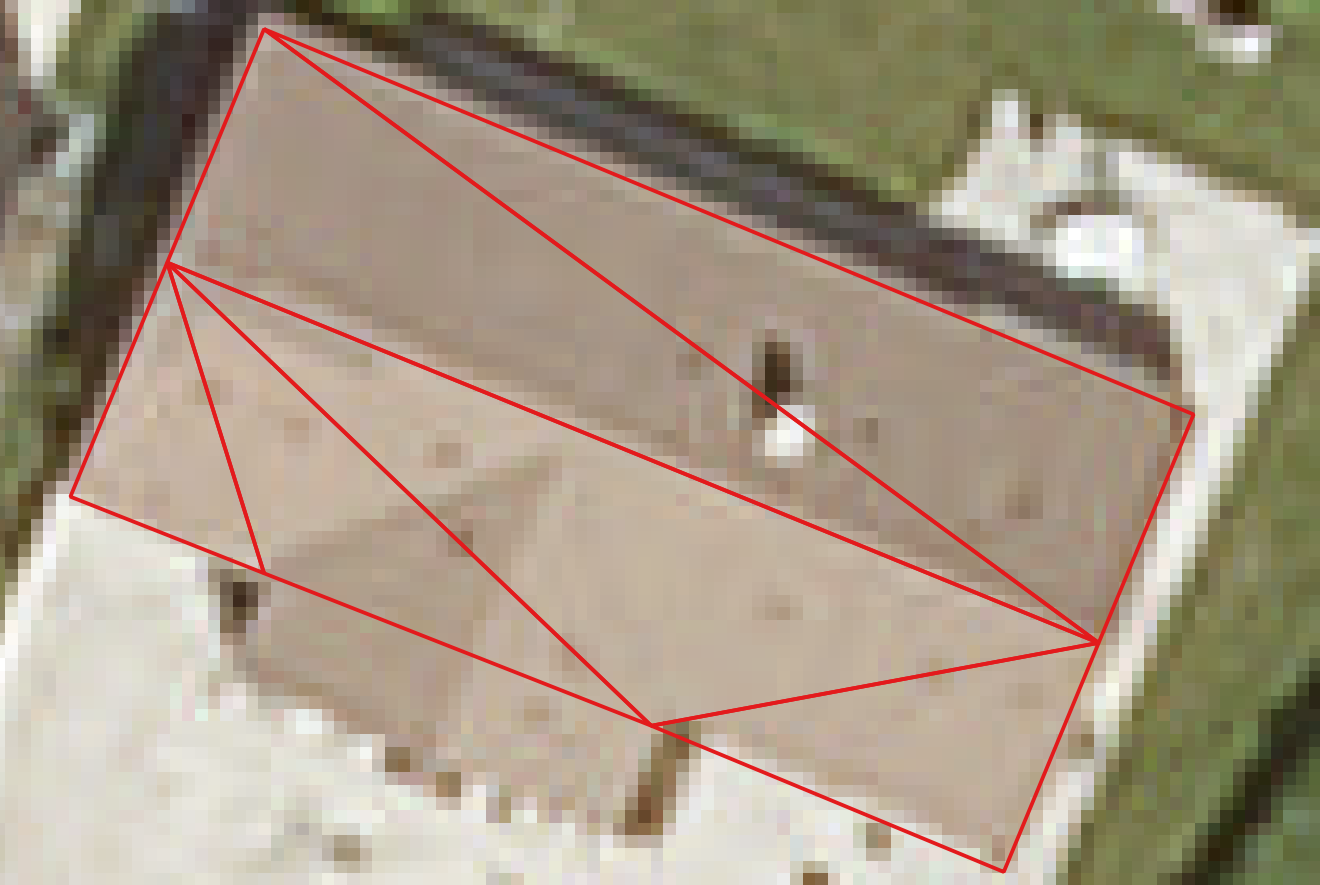
\includegraphics[width=.24\textwidth]{../images/raster/Facet_Errors/mis_segmentation}}}
						\ffigbox[\FBwidth]{\caption{Slope: Wrong facet slope.}\label{fig::slope}}{\fbox{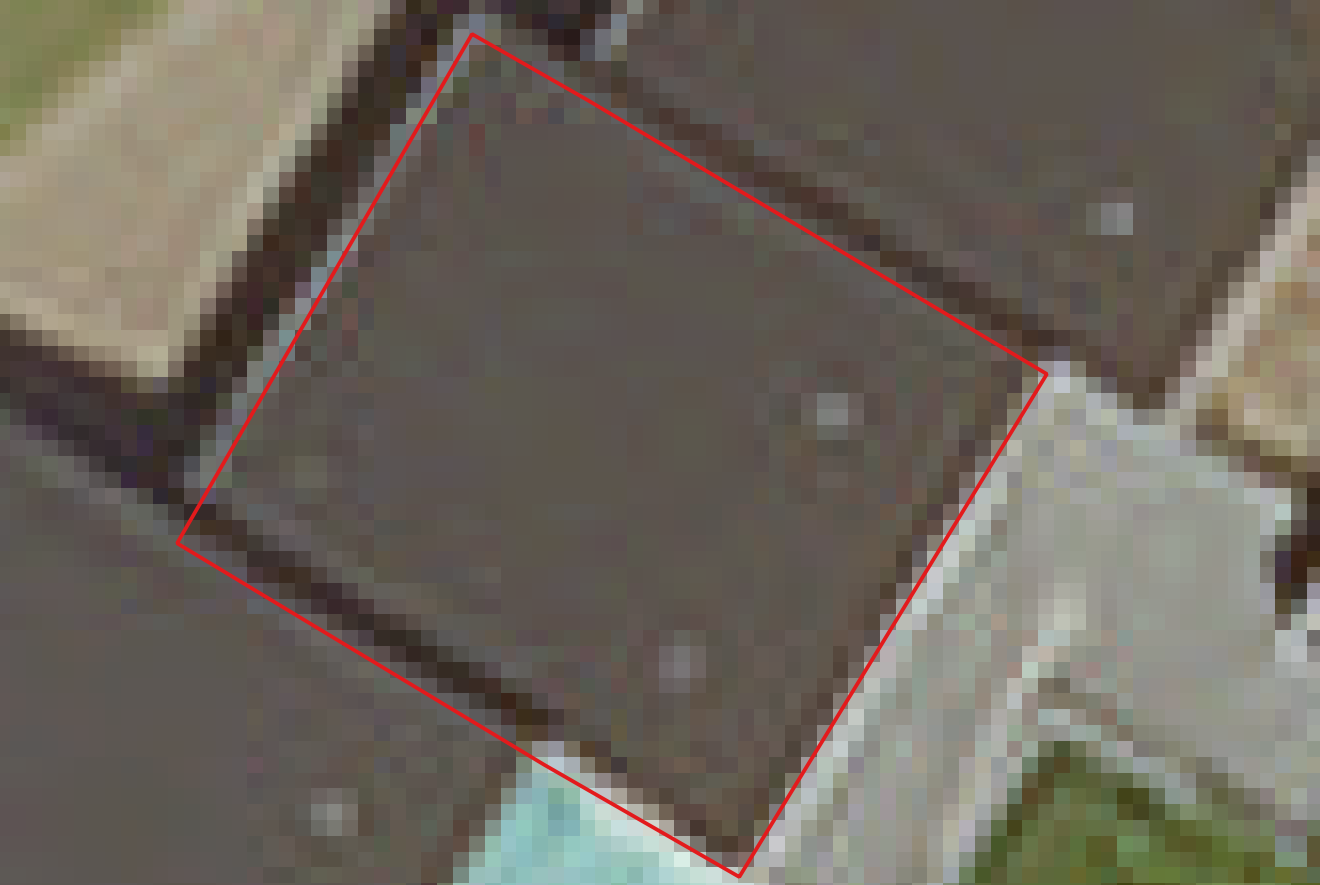
\includegraphics[width=.24\textwidth]{../images/raster/Facet_Errors/slope}}}
					\end{subfloatrow}
				}
				{
					\caption*{\label{fig::fac_samples} (iii). Samples of Facet errors.}
				}
			}
			{
				\caption{\label{fig::samples}Illustration of errors per class.}
			}
		\end{center}
	\end{figure}
	\clearpage


	Here are some statistics over the labelled dataset comprizing $502$ buildings:

	\begin{itemize}
		\item Ratio of \textbf{Building} errors among all errors: $0.2408$
		\begin{itemize}
			\item[-] Ratio of \textbf{Over Segmentation} errors:
			\begin{itemize}
				\item[(i).] among \textbf{Building} errors:  $0.1365$
				\item[(ii).] among all files:  $0.03287$
			\end{itemize}
			\item[-] Ratio of \textbf{Under Segmentation} errors:
			\begin{itemize}
				\item[(i).] among \textbf{Building} errors:  $0.4177$
				\item[(ii).] among all files:   $0.1006$
			\end{itemize}
			\item[-] Ratio of \textbf{Footprint} errors:
			\begin{itemize}
				\item[(i).] among \textbf{Building} errors:  $0.4839$
				\item[(ii).] among all files:  $0.1165$
			\end{itemize}
			\item[-] Ratio of \textbf{Altimetric} errors:
			\begin{itemize}
				\item[(i).] among \textbf{Building} errors:  $0.0165$
				\item[(ii).] among all files:  $0.0040$
			\end{itemize}
		\end{itemize}
		\item Ratio of \textbf{Facet} errors among all errors: $0.81657$
		\begin{itemize}
			\item[-] Ratio of \textbf{Over Segmentation} errors:
			\begin{itemize}
				\item[(i).] among \textbf{Facet} errors:  $0.8830$
				\item[(ii).] among all files:  $0.7203$
			\end{itemize}
			\item[-] Ratio of \textbf{Under Segmentation} errors:
			\begin{itemize}
				\item[(i).] among \textbf{Facet} errors:  $0.0842$
				\item[(ii).] among all files:   $0.0687$
			\end{itemize}
			\item[-] Ratio of \textbf{Mis Segmentation} errors:
			\begin{itemize}
				\item[(i).] among \textbf{Facet} errors:  $0.0806$
				\item[(ii).] among all files:  $0.0657$
			\end{itemize}
			\item[-] Ratio of \textbf{Slope} errors:
			\begin{itemize}
				\item[(i).] among \textbf{Facet} errors:  $0.0327$
				\item[(ii).] among all files:  $0.0267$
			\end{itemize}
		\end{itemize}
		\item Ratio of \textbf{Unqualified} errors among all errors: $0.0876$
		\begin{itemize}
			\item[-] Ratio of \textbf{Half Building} errors:
			\begin{itemize}
				\item[(i).] among \textbf{Unqualified} errors:  $0.8636$
				\item[(ii).] among all files:  $0.0757$
			\end{itemize}
			\item[-] Ratio of \textbf{Change Building} errors:
			\begin{itemize}
				\item[(i).] among \textbf{Unqualified} errors:  $0.0455$
				\item[(ii).] among all files:   $0.0040$
			\end{itemize}
			\item[-] Ratio of \textbf{Occlusion} errors:
			\begin{itemize}
				\item[(i).] among \textbf{Unqualified} errors:  $0.0455$
				\item[(ii).] among all files:  $0.0040$
			\end{itemize}
			\item[-] Ratio of \textbf{Unknown} errors:
			\begin{itemize}
				\item[(i).] among \textbf{Unqualified} errors:   $0.0455$
				\item[(ii).] among all files:  $0.0040$
			\end{itemize}
		\end{itemize}
	\end{itemize}


	\begin{landscape}
		\begin{figure}
			\begin{center}
				\includestandalone[mode=buildnew, scale=.78]{mind_map}
				\caption{\label{fig::mindmap_errors} Mind map summarizing the errors encountered during annotation.}
			\end{center}
		\end{figure}
	\end{landscape}

	\section{Features:}
~\\

	The first step of computing features was to extract low level features and
	expose them so that I can engineer sophisticated features to train the
	classifiers on. In fact, For each building, I computed the facet adjacency
	graph with meaningful information for each facet.

	\begin{figure}[H]
		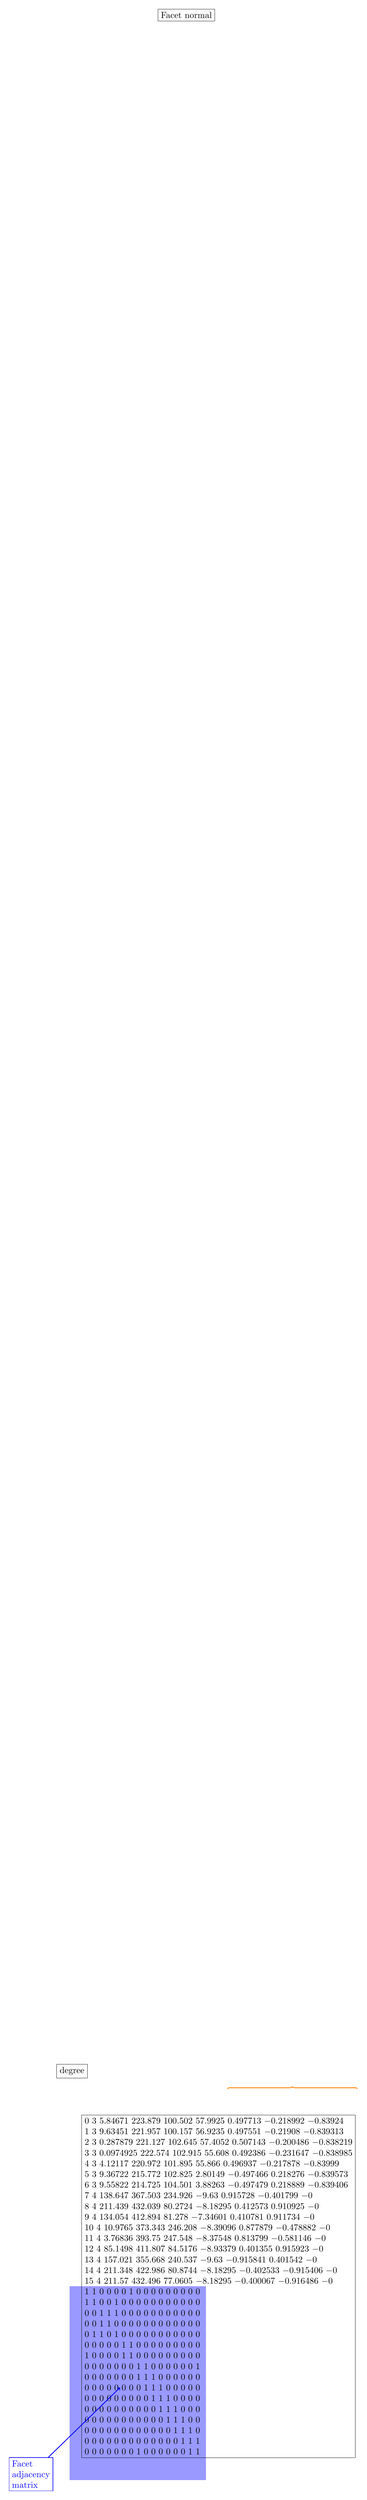
\begin{tikzpicture}
			\fill[blue!40] (-5.9,0) rectangle (-.5,-7.65);
			\node[draw, align=left] (feature)
			{
				$0$ $3$ $5.84671$ $223.879$ $100.502$ $57.9925$ $0.497713$ $-0.218992$ $-0.83924$\\
				$1$ $3$ $9.63451$ $221.957$ $100.157$ $56.9235$ $0.497551$ $-0.21908$ $-0.839313$\\
				$2$ $3$ $0.287879$ $221.127$ $102.645$ $57.4052$ $0.507143$ $-0.200486$ $-0.838219$\\
				$3$ $3$ $0.0974925$ $222.574$ $102.915$ $55.608$ $0.492386$ $-0.231647$ $-0.838985$\\
				$4$ $3$ $4.12117$ $220.972$ $101.895$ $55.866$ $0.496937$ $-0.217878$ $-0.83999$\\
				$5$ $3$ $9.36722$ $215.772$ $102.825$ $2.80149$ $-0.497466$ $0.218276$ $-0.839573$\\
				$6$ $3$ $9.55822$ $214.725$ $104.501$ $3.88263$ $-0.497479$ $0.218889$ $-0.839406$\\
				$7$ $4$ $138.647$ $367.503$ $234.926$ $-9.63$ $0.915728$ $-0.401799$ $-0$\\
				$8$ $4$ $211.439$ $432.039$ $80.2724$ $-8.18295$ $0.412573$ $0.910925$ $-0$\\
				$9$ $4$ $134.054$ $412.894$ $81.278$ $-7.34601$ $0.410781$ $0.911734$ $-0$\\
				$10$ $4$ $10.9765$ $373.343$ $246.208$ $-8.39096$ $0.877879$ $-0.478882$ $-0$\\
				$11$ $4$ $3.76836$ $393.75$ $247.548$ $-8.37548$ $0.813799$ $-0.581146$ $-0$\\
				$12$ $4$ $85.1498$ $411.807$ $84.5176$ $-8.93379$ $0.401355$ $0.915923$ $-0$\\
				$13$ $4$ $157.021$ $355.668$ $240.537$ $-9.63$ $-0.915841$ $0.401542$ $-0$\\
				$14$ $4$ $211.348$ $422.986$ $80.8744$ $-8.18295$ $-0.402533$ $-0.915406$ $-0$\\
				$15$ $4$ $211.57$ $432.496$ $77.0605$ $-8.18295$ $-0.400067$ $-0.916486$ $-0$\\
				1 1 0 0 0 0 1 0 0 0 0 0 0 0 0 0\\
				1 1 0 0 1 0 0 0 0 0 0 0 0 0 0 0\\
				0 0 1 1 1 0 0 0 0 0 0 0 0 0 0 0\\
				0 0 1 1 0 0 0 0 0 0 0 0 0 0 0 0\\
				0 1 1 0 1 0 0 0 0 0 0 0 0 0 0 0\\
				0 0 0 0 0 1 1 0 0 0 0 0 0 0 0 0\\
				1 0 0 0 0 1 1 0 0 0 0 0 0 0 0 0\\
				0 0 0 0 0 0 0 1 1 0 0 0 0 0 0 1\\
				0 0 0 0 0 0 0 1 1 1 0 0 0 0 0 0\\
				0 0 0 0 0 0 0 0 1 1 1 0 0 0 0 0\\
				0 0 0 0 0 0 0 0 0 1 1 1 0 0 0 0\\
				0 0 0 0 0 0 0 0 0 0 1 1 1 0 0 0\\
				0 0 0 0 0 0 0 0 0 0 0 1 1 1 0 0\\
				0 0 0 0 0 0 0 0 0 0 0 0 1 1 1 0\\
				0 0 0 0 0 0 0 0 0 0 0 0 0 1 1 1\\
				0 0 0 0 0 0 0 1 0 0 0 0 0 0 1 1
			};
			\node[draw, align=left, below left of=feature, node distance=10.5cm, blue] (matrix)
			{
				Facet\\adjacency\\matrix
			};
			\draw[->, line width=.3mm, blue] (matrix) edge (-3.9,-4);
			\node[draw] (degree) at (-5.8, 8.5) {degree};
			\draw[decorate, line width=.3mm, decoration={brace}, orange]  (.35, 7.8) -- (5.5, 7.8);
			\node[draw] (normal) at (2,93, 8.5) {Facet normal};
		\end{tikzpicture}
	\end{figure}

	\section*{Attachments:}
	\begin{itemize}
		\item[-] You can checkout the preprocessing code on
		\href{https://github.com/ethiy/proj.city}{Github}.
		\item[-] You can also check the feature extraction and classification code
		\href{https://github.com/ethiy/qualcity}{here}.
	\end{itemize}

\end{document}
